\section{Electron}
\label{sec:electron}
Electron originally was released as Atom Shell by GitHub at \displaydate{dateAtomShell}~\cite{githubReleaseV010} and downloaded approx. $83\,000\,000$ times\footnote{According to \url{https://npm-stat.com/charts.html?package=electron&from=2013-07-13&to=2022-07-30}}
The intention of the developers was ``to handle the Chromium/Node.js event loop integration and native APIs``~\cite{sawicki_2015} for the Atom Editor.
On \displaydate{dateRenameElectron} it was renamed to Electron and announced that the developers want to provide a framework that allows to build desktop applications with the using web-technologies.
Many day-to-day apps have been implemented using Electron like Discord, Twitch or even Microsoft Teams.
This has lead to an increasing community which can be expressed numerically based on GitHub Statistics~\cite{GithubElectron} \\ \\:
\begin{tabular} {| c | c | c | c | c |}
    \label{tab:electron:statistics}
    Stars      & Forks     & Watching & Used by    & Contributors \\ \hline
    $130\,000$ & $13\,700$ & $2\,900$ & $244\,568$ & $1\,126$
\end{tabular}

\subsection{Architecture}
\label{subsec:electron:architecture}
Electrons architecture fundamentally relies on Chromium, an open-source browser which is included in each Electron executable and has a lot common with it.
As Chromium Electron is based on a multi-process model, containing of a single process called \textbf{main} and several processes, one for each window, called \textbf{renderer}
\begin{figure}[ht]
    \label{fig:electron:model}
    \centering
    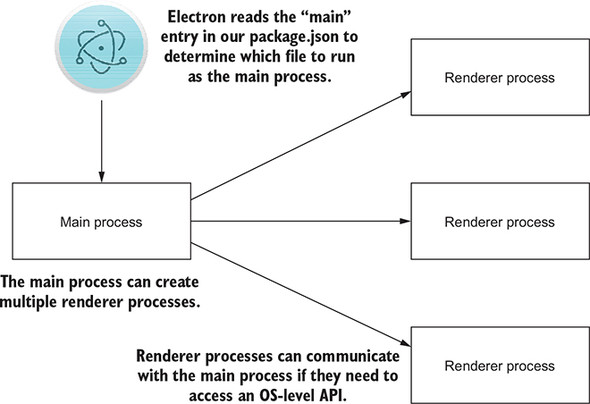
\includegraphics[width=0.4\textwidth]{images/electron-model}
    \caption[Bla]{Multi-process Model Electron from~\cite[Fig. 1.7]{electron-in-action}}
\end{figure}
\begin{description}
    \item[\textbf{Main}:] \hfill \\ This is the main entry point of the application and responsible for lifecycle management like starting or quitting the app.
    The \texttt{main} process uses so called \texttt{BrowserWindow} module to create and manage each \texttt{renderer} process which is loading web pages into it.
    Since just the \texttt{main} process is running inside a NodeJS environment, it is the only part of the application that can import NodeJS modules using \texttt{require}.
    This forces each \texttt{renderer} process to interact with the \texttt{main} process if they want to consume system \ac{API}s for purposes like saving files or opening dialogs.
    \item[\textbf{Renderer}:] \hfill \\ As it is implied by the name a \texttt{renderer} process renders web content by loading web pages into it and presenting them to the user.
    Additionally, javascript code can be loaded and executed inside a process.
    Each \texttt{renderer} process can be created or destroyed by the main process using the \texttt{BrowserWindow} module as mentioned before.
    This leads to the fact, that \texttt{renderer} processes are isolated from each other following the Chromium principles of a multi-process model and is reasoned by limited affection of
    faulty or malicious code on the entire app.
    The \texttt{renderer} processes are only able to communicate between each other indirectly via the \texttt{main} process.
    This is called \ac{IPC}
\end{description}

\subsubsection{IPC}
As mentioned above \texttt{main} and \texttt{main} processes are only able to communicate using \ac{IPC}.
Therefor Electron provides two modules, one for the \texttt{main} process, called \texttt{ipcMain} and one for \texttt{renderer} process, called \texttt{ipcRender}.
Both of them are Node.JS \texttt{eventEmitter} modules and capable of executing asynchronously and synchronously communication either uni- or bidirectional.

\subsubsection{Context Isolation}
Electrons multi-process model also intends distinct purposes for each process.
As described before only the \texttt{main} process has access to node modules.
In contrast to that only the \texttt{renderer} process has access to \ac{HTML} \ac{DOM}s.
Since using just \ac{IPC} represents a major security issue, Electron introduced a feature called \textbf{Context Isolation}.
This splits the logic of a \texttt{renderer} process into two different contexts on the one hand the \texttt{renderer} process as already described and on the other a so called \texttt{preload script}.
The \texttt{preload script} is attached to the \texttt{main} process at the creation of the \texttt{BrowserWindow} module and at its context has access to both node modules and \ac{HTML} \ac{DOM}s.
Although the \texttt{preload script} and the \texttt{renderer} process do both own a window object which provides the displayed browser window it is not the same object since they are both running at
different contexts.
The \texttt{preload script} consists of a \texttt{contextBridge} module which is responsible for safely exposing selected properties of the \texttt{main} process to the \texttt{renderer} and vice versa.
Inside this module an \ac{API} can be defined for providing access with \ac{IPC} objects to resources of different processes.

%each view is rendered at a separate process, called \textbf{renderer}.
%The reason for this is that faulty or malicious code is limited in its affection at the whole app.
%Each process is controlled by a single process, which is also the entry point of the app, called \textbf{main}.

\subsection{Frontend}
\label{subsec:electron:frontend}
This subsection deals with the front-end Electron is using, which other frontend-frameworks are supported, etc.

\subsection{Backend}
\label{subsec:electron:backend}
At this subsection we will take a look at the Node JS Backend of Electron and analyse the advantages and disadvantages of NodeJS